\documentclass[aspectratio=169,10pt]{beamer}

\usepackage[T1]{fontenc}
\usepackage{lmodern}
\usepackage{amsmath,amssymb}
\usepackage{booktabs}
\usepackage{array}
\usepackage{tikz}
\usetikzlibrary{arrows.meta, backgrounds, calc, fit, positioning, shapes.geometric}
\usepackage{xcolor}

\definecolor{potsdamblue}{HTML}{00315E}
\definecolor{panelblue}{HTML}{E7F0F6}
\definecolor{lineblue}{HTML}{A9C0D5}
\definecolor{softgreen}{HTML}{EAF6EC}
\definecolor{softgold}{HTML}{FFF3D6}
\definecolor{softgray}{HTML}{F6F8FA}
\definecolor{textgray}{HTML}{1B2A34}

\setbeamercolor{normal text}{fg=textgray}
\setbeamercolor{frametitle}{fg=white,bg=potsdamblue}
\setbeamercolor{title}{fg=white}
\setbeamercolor{author}{fg=white}
\setbeamercolor{block title}{fg=white,bg=potsdamblue}
\setbeamercolor{block body}{fg=textgray,bg=panelblue}
\setbeamercolor{itemize item}{fg=potsdamblue}
\setbeamercolor{itemize subitem}{fg=potsdamblue}
\setbeamertemplate{navigation symbols}{}
\setbeamertemplate{itemize item}{\textbullet}
\setbeamertemplate{itemize subitem}{\textendash}

\setbeamertemplate{frametitle}{%
  \nointerlineskip
  \begin{beamercolorbox}[wd=\paperwidth,ht=0.95cm,dp=0.25cm,leftskip=0.4cm,rightskip=0.4cm]{frametitle}
    \vspace{2pt}\bfseries\large\insertframetitle
  \end{beamercolorbox}
}

\newcommand{\sectionhead}[1]{%
  \vspace{2pt}%
  \colorbox{potsdamblue}{\color{white}\bfseries\strut~#1~}%
  \par\vspace{2pt}%
}

\title{LAMP: ASP Rule Induction and Optimization with LLMs}
\author{David Bunker}
\institute{University of Potsdam}
\date{}

\begin{document}

\begin{frame}{LAMP\quad LLM to ASP Modeling Protocol}

\begin{columns}[T,onlytextwidth]

\begin{column}{0.52\textwidth}

\sectionhead{Task}
\footnotesize
ASP rule induction. Given facts $F$ and a target answer set $A^*$, find a small program $\Pi$ with
\[
  AS(F \cup \Pi) = \{A^*\}.
\]
Bounded unary normal rules.

\vspace{0.15cm}
\sectionhead{Loop}
\footnotesize
\begin{itemize}\itemsep1pt
  \item LLM proposes rules from $F$, $A^*$, schema bounds.
  \item \textsc{Clingo} verifies the stable model.
  \item Mismatches feed back. Up to 3 attempts.
  \item No fine tuning. Solver decides correctness.
\end{itemize}

\vspace{0.15cm}
\sectionhead{Setup}
\footnotesize
120 synthetic benchmarks varying predicates, terms, facts, body literals, negation, derived atoms. ILASP baseline runs conflict driven search over an ASP meta encoding, 7 min timeout.

\end{column}

\begin{column}{0.46\textwidth}

\sectionhead{Iterative Loop}
\centering
\resizebox{0.98\linewidth}{!}{%
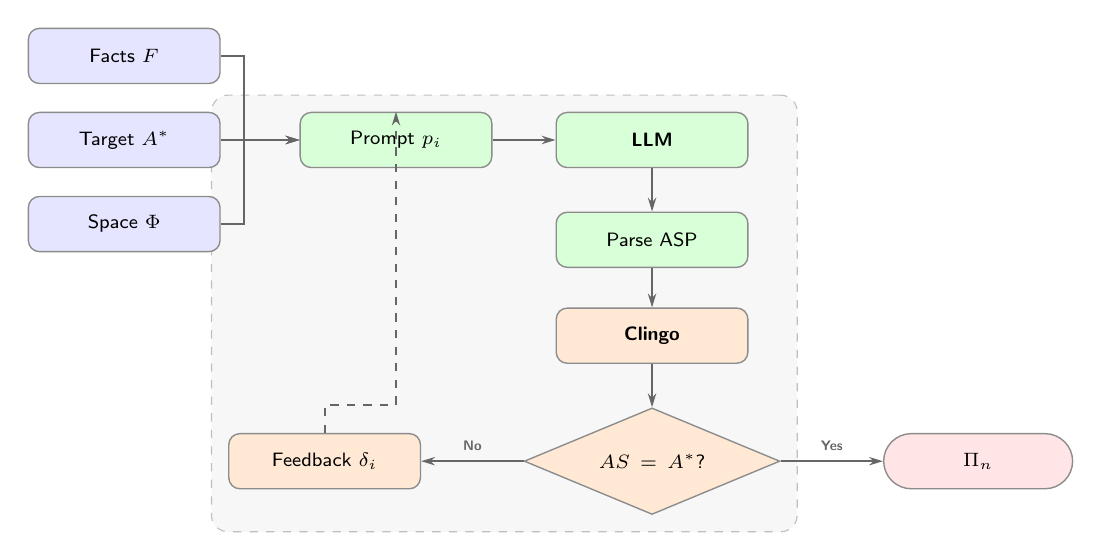
\begin{tikzpicture}[node distance=0.35cm and 0.85cm]
  \colorlet{inputcol}{blue!10}
  \colorlet{llmcol}{green!15}
  \colorlet{clingocol}{orange!17}
  \colorlet{outcol}{red!10}
  \colorlet{loopbg}{black!3}
  \tikzset{
    proc/.style={rectangle, rounded corners=4pt,
      minimum width=2.4cm, minimum height=0.7cm,
      text centered, text width=2.2cm,
      font=\sffamily\scriptsize,
      draw=black!45, line width=0.5pt, fill=#1},
    proc/.default=white,
    decision/.style={diamond, aspect=2.4,
      minimum width=2.6cm, minimum height=0.75cm,
      text centered, text width=2.0cm,
      font=\sffamily\scriptsize,
      draw=black!45, line width=0.5pt, fill=clingocol},
    terminal/.style={rectangle, rounded corners=10pt,
      minimum width=2.4cm, minimum height=0.7cm,
      text centered, text width=2.1cm,
      font=\sffamily\scriptsize\bfseries,
      draw=black!45, line width=0.5pt, fill=#1},
    terminal/.default=outcol,
    arr/.style={-{Stealth[length=5pt, width=3pt]}, line width=0.8pt, color=black!60},
    darr/.style={-{Stealth[length=5pt, width=3pt]}, line width=0.7pt, color=black!60, dashed}
  }
  \node[proc=inputcol] (facts) {Facts $F$};
  \node[proc=inputcol, below=of facts] (target) {Target $A^*$};
  \node[proc=inputcol, below=of target] (space) {Space $\Phi$};
  \node[proc=llmcol, right=1.0cm of target] (prompt) {Prompt $p_i$};
  \node[proc=llmcol, right=0.8cm of prompt] (llm) {\textbf{LLM}};
  \node[proc=llmcol, below=0.55cm of llm] (parse) {Parse ASP};
  \node[proc=clingocol, below=0.5cm of parse] (clingo) {\textbf{Clingo}};
  \node[decision, below=0.55cm of clingo] (check) {$AS = A^*$?};
  \node[proc=clingocol, left=1.3cm of check] (feedback) {Feedback $\delta_i$};
  \node[terminal=outcol, right=1.3cm of check] (out) {$\Pi_n$};
  \begin{scope}[on background layer]
    \node[draw=black!25, dashed, rounded corners=6pt, fill=loopbg,
      fit=(prompt)(llm)(parse)(clingo)(check)(feedback), inner sep=6pt] {};
  \end{scope}
  \draw[arr] (facts.east) -- ++(0.30,0) |- (prompt.west);
  \draw[arr] (target.east) -- (prompt.west);
  \draw[arr] (space.east) -- ++(0.30,0) |- (prompt.west);
  \draw[arr] (prompt.east) -- (llm.west);
  \draw[arr] (llm.south) -- (parse.north);
  \draw[arr] (parse.south) -- (clingo.north);
  \draw[arr] (clingo.south) -- (check.north);
  \draw[arr] (check.east) -- node[above, font=\sffamily\tiny\bfseries]{Yes} (out.west);
  \draw[arr] (check.west) -- node[above, font=\sffamily\tiny\bfseries]{No} (feedback.east);
  \draw[darr] (feedback.north) -- ++(0,0.35) -| (prompt.north);
\end{tikzpicture}%
}

\vspace{0.15cm}
\sectionhead{Results across 120 benchmarks}
\centering
\footnotesize
\renewcommand{\arraystretch}{1.05}
\begin{tabular}{@{}lrrr@{}}
\toprule
\textbf{System} & \textbf{1st} & \textbf{Final} & \textbf{Fails} \\
\midrule
\textit{gpt-5-mini}     & 90.8\% & 99.2\% & 1  \\
\textit{gpt-oss}    & 83.3\% & 98.3\% & 2  \\
\textit{qwen3-coder}    & 19.2\% & 64.2\% & 43 \\
ILASP                   & ---    & 97.5\% & 3  \\
\bottomrule
\end{tabular}

\vspace{0.10cm}
{\scriptsize Output literals 3 to 6 vs 22 or 33 originals. Stratified 119/119, 117/118, 117/117 vs 49/120 originals.\par}

\end{column}
\end{columns}

\vspace{0.15cm}
\begin{beamercolorbox}[wd=\textwidth,sep=4pt,rounded=true]{block body}
\centering\footnotesize
Both strong LAMP models solved all 3 ILASP timeout benchmarks. Outputs were smaller and fully stratified. Natural extension: hybridize ILASP search with an agentic LLM loop on richer benchmarks like ASPBench.
\end{beamercolorbox}

\end{frame}

\end{document}
